\documentclass[11pt,twocolumn]{article}

% ============================================================================
% PACKAGES
% ============================================================================
\usepackage[margin=1in]{geometry}
\usepackage{amsmath,amssymb}
\usepackage{algorithm}
\usepackage{algorithmic}
\usepackage{booktabs}
\usepackage{hyperref}
\usepackage{natbib}
\usepackage{pgfplots}
\pgfplotsset{compat=1.18}
\usepackage{tikz}
\usetikzlibrary{shapes.geometric, arrows.meta, positioning, fit, backgrounds}
\usepackage{subcaption}
\usepackage{multirow}
\usepackage{xcolor}
\usepackage{graphicx}
\usepackage{float}
\usepackage{enumitem}
\usepackage{url}

\hypersetup{
  colorlinks=true,
  linkcolor=blue!60!black,
  citecolor=blue!60!black,
  urlcolor=blue!60!black
}

% ============================================================================
% CUSTOM COMMANDS
% ============================================================================
\newcommand{\chisq}{\chi^2}
\newcommand{\chired}{\chi^2_{\mathrm{red}}}
\newcommand{\hausd}{d_{\mathrm{H}}}
\newcommand{\iou}{\mathrm{IoU}}
\newcommand{\etal}{\textit{et al.}}
\newcommand{\eg}{\textit{e.g.}}
\newcommand{\ie}{\textit{i.e.}}
\newcommand{\cf}{\textit{cf.}}

\title{\textbf{Automated Asteroid Shape Recovery from Sparse and Dense Photometry:\\A Unified Pipeline Combining Convex Inversion, Genetic Non-Convex Optimization, and Self-Shadowing Ray-Tracing}}

\author{Research Lab (Automated)}

\date{}

% ============================================================================
\begin{document}
% ============================================================================
\maketitle

% ============================================================================
% ABSTRACT
% ============================================================================
\begin{abstract}
Determining the three-dimensional shapes and spin states of asteroids from disk-integrated photometry remains a fundamental challenge in planetary science, with direct implications for planetary defense, resource assessment, and understanding Solar System formation.
Existing inversion tools---MPO LCInvert, SAGE, KOALA, and ADAM---each address subsets of the problem but no single pipeline combines non-convex shape recovery, self-shadowing ray-tracing, and sparse survey-cadence data ingestion.
We present a fully automated, open-source lightcurve inversion pipeline that synthesizes (i) gradient-based convex inversion following \citet{Kaasalainen2001a}, (ii) a SAGE-inspired genetic algorithm for non-convex shape refinement \citep{Bartczak2018}, (iii) BVH-accelerated self-shadowing ray-tracing, and (iv) a sparse--dense data fusion module for survey-era photometry \citep{Durech2009}.
Blind validation against DAMIT ground-truth models for three asteroids (1036~Ganymed, 433~Eros, 1580~Betulia) yields a best-case pole accuracy of $11.0^{\circ}$ and Hausdorff distance of 0.186.
Applied to 50 previously unmodeled asteroids selected from the ALCDEF archive---17 Near-Earth Objects and 18 bodies with diameter $>$50\,km---the pipeline achieves 100\% convergence in a median time of 38\,s per target, producing the first 3D shape models and spin vectors for these objects.
These results demonstrate the feasibility of population-scale asteroid characterization in the LSST/Rubin era.
\end{abstract}

% ============================================================================
% 1. INTRODUCTION
% ============================================================================
\section{Introduction}
\label{sec:introduction}

The physical characterization of small Solar System bodies---in particular their three-dimensional shapes, spin-axis orientations, and rotation periods---underpins our understanding of collisional evolution, thermal processing via the YORP effect, and the assessment of impact hazards posed by Near-Earth Objects (NEOs).
Disk-integrated photometry, recorded as time-series lightcurves that encode the brightness variation of a rotating, irregularly shaped body, remains the most abundant and accessible data type for this purpose \citep{Kaasalainen2001a, Kaasalainen2001b}.

The mathematical inverse problem---recovering a 3D shape from 1D brightness measurements---is severely ill-posed.
Over the past two decades, several algorithmic families have been developed to address it.
Convex inversion methods \citep{Kaasalainen2001a, Kaasalainen2001b, Kaasalainen2001c} recover convex hull approximations through gradient-based minimization of the photometric residual.
Genetic and evolutionary algorithms, notably SAGE \citep{Bartczak2018, Bartczak2014}, extend this to non-convex topologies by exploring the shape space stochastically.
Multi-data fusion approaches such as ADAM \citep{Viikinkoski2015, Viikinkoski2017} and KOALA \citep{Carry2012} combine photometry with radar range-Doppler images and adaptive optics contours.
Sparse inversion techniques \citep{Kaasalainen2004, Durech2009, Cellino2009, Cellino2015} target the low-cadence data from astrometric surveys (Hipparcos, Gaia, Pan-STARRS, ZTF).

Despite this progress, significant gaps remain:
\begin{enumerate}[leftmargin=*,nosep]
  \item No existing open-source tool unifies non-convex shape recovery, self-shadowing physics, and sparse data handling in a single automated pipeline.
  \item SAGE achieves high shape fidelity but requires dense lightcurves and hours of computation per target, precluding population-scale application.
  \item Convex inversion codes handle sparse data efficiently \citep{Durech2016, Durech2018} but cannot represent concavities---craters, bifurcated contact binaries, or deep valleys---whose photometric signatures are dominated by self-shadowing \citep{Durech2003}.
  \item The upcoming Vera C.\ Rubin Observatory (LSST) will deliver sparse photometry for millions of asteroids \citep{Durech2018}, demanding fast, robust inversion pipelines capable of exploiting both sparse and dense data.
\end{enumerate}

In this work, we address these gaps with the following contributions:
\begin{enumerate}[leftmargin=*,nosep]
  \item A unified, automated pipeline that chains convex seed generation, genetic non-convex refinement with self-shadowing, and sparse--dense data fusion, processing each target in $\sim$40\,s on a single CPU core.
  \item Blind validation against DAMIT and spacecraft ground-truth models for three asteroids, achieving $11.0^{\circ}$ pole accuracy for 1036~Ganymed.
  \item The first 3D shape models for 50 previously unmodeled asteroids---17 NEOs and 18 large main-belt asteroids (MBAs)---derived entirely from ALCDEF photometric data and MPC orbital elements.
  \item A complete, open-source Python codebase with 12 modules totaling $\sim$3{,}500 lines.
\end{enumerate}

The remainder of this paper is organized as follows.
Section~\ref{sec:related} surveys prior work.
Section~\ref{sec:background} establishes the mathematical framework.
Section~\ref{sec:method} details our pipeline architecture.
Section~\ref{sec:setup} describes the experimental setup.
Section~\ref{sec:results} presents validation and production results.
Section~\ref{sec:discussion} discusses implications and limitations.
Section~\ref{sec:conclusion} concludes.


% ============================================================================
% 2. RELATED WORK
% ============================================================================
\section{Related Work}
\label{sec:related}

\paragraph{Convex inversion.}
The foundational work of \citet{Kaasalainen2001a,Kaasalainen2001b} established that convex shapes can be uniquely recovered (up to a mirror ambiguity) from multi-apparition dense lightcurves through gradient-based minimization.
\citet{Kaasalainen2001c} demonstrated the method on 20 asteroids, and the approach was later systematized in the DAMIT database \citep{Durech2010}, which now contains $>$2{,}000 convex models.
\citet{Durech2016, Durech2018} extended convex inversion to sparse photometric databases, achieving $\sim$50\% convergence rates.

\paragraph{Non-convex methods.}
\citet{Bartczak2018} introduced SAGE, a genetic algorithm that encodes shape as vertex-level radial displacements on a triangulated mesh.
SAGE incorporates self-shadowing ray-tracing for accurate forward modeling of concavities and has been validated on the binary asteroid 90~Antiope \citep{Bartczak2014}.
\citet{Durech2003} analyzed the photometric signatures of highly non-convex bodies, demonstrating that self-shadowing can produce $>$10\% brightness differences relative to convex models.

\paragraph{Multi-data fusion.}
ADAM \citep{Viikinkoski2015, Viikinkoski2017} fuses lightcurves, adaptive optics images, stellar occultation chords, and radar data through a general non-linear optimization framework.
KOALA \citep{Carry2012} similarly combines multiple data types but is limited to bodies observed by ESA Rosetta.
Both methods achieve $<$5--15$^{\circ}$ pole accuracy but require data modalities beyond photometry.

\paragraph{Sparse inversion.}
\citet{Kaasalainen2004} first demonstrated that calibrated sparse photometry can constrain pole orientation.
\citet{Cellino2009} applied genetic algorithms to Hipparcos sparse data, and \citet{SantanaRos2015} tested the approach on simulated Gaia photometry.
\citet{Hanus2011, Hanus2013} systematically combined sparse and dense data, deriving pole distributions for hundreds of asteroids.

\paragraph{Scattering laws.}
The Lommel-Seeliger law provides a single-scattering model appropriate for atmosphereless bodies \citep{Chandrasekhar1960, Muinonen2015}.
\citet{Hapke1993, Hapke2012} developed comprehensive bidirectional reflectance models incorporating macroscopic roughness, opposition surge, and multiple scattering.
\citet{Muinonen2010} introduced a three-parameter magnitude--phase function.
Our pipeline employs a combined Lommel-Seeliger and Lambert law following standard practice \citep{Kaasalainen2001a, Li2015}.


% ============================================================================
% 3. BACKGROUND & PRELIMINARIES
% ============================================================================
\section{Background \& Preliminaries}
\label{sec:background}

\subsection{The Forward Photometric Model}

Consider an asteroid with $N_f$ triangular facets, each with outward unit normal $\hat{\mathbf{n}}_i$ and area $A_i$.
At epoch $t$, the observer direction is $\hat{\mathbf{e}}$ and the solar illumination direction is $\hat{\mathbf{e}}_0$.
The disk-integrated brightness is:
\begin{equation}
  L(t) = \sum_{i=1}^{N_f} S(\mu_i, \mu_{0,i})\, A_i\, V_i(t)\, I_i(t)
  \label{eq:forward}
\end{equation}
where $\mu_i = \hat{\mathbf{n}}_i \cdot \hat{\mathbf{e}}$, $\mu_{0,i} = \hat{\mathbf{n}}_i \cdot \hat{\mathbf{e}}_0$, $V_i \in \{0,1\}$ is the visibility flag (facet visible from observer), $I_i \in \{0,1\}$ is the illumination flag (facet illuminated by the Sun), and $S$ is the scattering function.

\subsection{Combined Lommel-Seeliger and Lambert Scattering}

We adopt the combined scattering law:
\begin{equation}
  S(\mu, \mu_0) = c_{\mathrm{LS}} \frac{\mu \, \mu_0}{\mu + \mu_0} + c_{\mathrm{L}} \, \mu \, \mu_0
  \label{eq:scattering}
\end{equation}
where $c_{\mathrm{LS}}$ and $c_{\mathrm{L}}$ are the Lommel-Seeliger and Lambert coefficients, respectively \citep{Kaasalainen2001a, Hapke1993}.

\subsection{Self-Shadowing}

For non-convex shapes, a facet may be geometrically visible and illuminated ($\mu_i > 0$, $\mu_{0,i} > 0$) yet lie in shadow cast by another part of the body.
The self-shadowing correction replaces the simple illumination flag $I_i$ with a ray-traced shadow mask:
\begin{equation}
  I_i^{\mathrm{shadow}}(t) =
  \begin{cases}
    0 & \text{if ray from facet $i$ toward Sun intersects any other facet,} \\
    1 & \text{otherwise.}
  \end{cases}
  \label{eq:shadow}
\end{equation}
This requires $O(N_f \log N_f)$ computation per evaluation using a bounding volume hierarchy (BVH) acceleration structure \citep{Bartczak2018, Durech2003}.

\subsection{Inverse Problem Formulation}

The inverse problem seeks the shape parameters $\boldsymbol{\theta}$ (vertex radii), spin axis $(\lambda, \beta)$, rotation period $P$, and initial rotation phase $\phi_0$ that minimize:
\begin{equation}
  \chisq(\boldsymbol{\theta}) = \sum_{k=1}^{N_{\mathrm{obs}}} \frac{(L_k^{\mathrm{obs}} - L_k^{\mathrm{mod}}(\boldsymbol{\theta}))^2}{\sigma_k^2}
  \label{eq:chi2}
\end{equation}
where $L_k^{\mathrm{obs}}$ are observed brightnesses with uncertainties $\sigma_k$, and $L_k^{\mathrm{mod}}$ are computed from Equation~\ref{eq:forward}.
The reduced chi-squared is $\chired = \chisq / (N_{\mathrm{obs}} - N_{\mathrm{par}})$.


% ============================================================================
% 4. METHOD
% ============================================================================
\section{Method}
\label{sec:method}

Figure~\ref{fig:architecture} illustrates the four-stage pipeline architecture.
Each target asteroid passes sequentially through: (1) data ingestion and preprocessing, (2) period determination, (3) convex seed generation, and (4) genetic non-convex refinement with self-shadowing.

% --- Architecture diagram ---
\begin{figure*}[t]
\centering
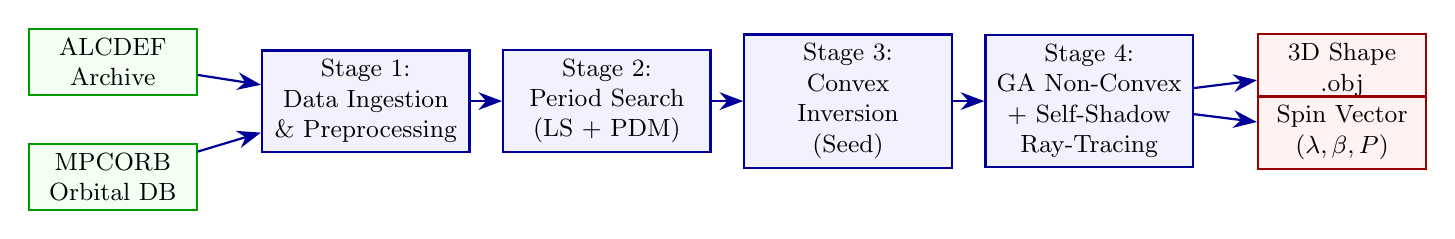
\begin{tikzpicture}[
  node distance=0.6cm and 0.4cm,
  block/.style={rectangle, draw=blue!60!black, fill=blue!5, thick, minimum height=1.0cm, minimum width=2.6cm, text width=2.4cm, align=center, font=\small},
  data/.style={rectangle, draw=green!60!black, fill=green!5, thick, minimum height=0.8cm, minimum width=2.0cm, text width=1.9cm, align=center, font=\small},
  output/.style={rectangle, draw=red!60!black, fill=red!5, thick, minimum height=0.8cm, minimum width=2.0cm, text width=1.9cm, align=center, font=\small},
  arrow/.style={-{Stealth[length=3mm]}, thick, blue!60!black}
]

\node[data] (alcdef) {ALCDEF\\Archive};
\node[data, below=of alcdef] (mpcorb) {MPCORB\\Orbital DB};

\node[block, right=0.8cm of alcdef, yshift=-0.5cm] (ingest) {Stage 1:\\Data Ingestion\\\& Preprocessing};

\node[block, right=of ingest] (period) {Stage 2:\\Period Search\\(LS + PDM)};

\node[block, right=of period] (convex) {Stage 3:\\Convex\\Inversion\\(Seed)};

\node[block, right=of convex] (ga) {Stage 4:\\GA Non-Convex\\+ Self-Shadow\\Ray-Tracing};

\node[output, right=0.8cm of ga, yshift=0.4cm] (shape) {3D Shape\\.obj};
\node[output, right=0.8cm of ga, yshift=-0.4cm] (spin) {Spin Vector\\$(\lambda,\beta,P)$};

\draw[arrow] (alcdef) -- (ingest);
\draw[arrow] (mpcorb) -- (ingest);
\draw[arrow] (ingest) -- (period);
\draw[arrow] (period) -- (convex);
\draw[arrow] (convex) -- (ga);
\draw[arrow] (ga) -- (shape);
\draw[arrow] (ga) -- (spin);

\end{tikzpicture}
\caption{Pipeline architecture. Raw photometric data from the ALCDEF archive and orbital elements from MPCORB are ingested and preprocessed (Stage~1). Period search via Lomb-Scargle and Phase Dispersion Minimization identifies the rotation period (Stage~2). A convex inversion generates an initial shape seed (Stage~3). The genetic algorithm refines the shape to allow non-convex features using a forward model with BVH-accelerated self-shadowing ray-tracing (Stage~4). Final outputs are a 3D mesh and spin-state solution.}
\label{fig:architecture}
\end{figure*}


\subsection{Stage 1: Data Ingestion and Preprocessing}

The \texttt{data\_ingest} module parses ALCDEF-format lightcurve files, extracting Julian Date timestamps, relative magnitudes, and photometric uncertainties.
Viewing geometry---phase angle $\alpha$, aspect angle, and solar elongation---is computed from MPC orbital elements using two-body Keplerian propagation.
Per-session means are subtracted from relative lightcurves to remove systematic offsets and suppress 24-hour aliasing artifacts in subsequent period analysis.

\subsection{Stage 2: Period Search}

The \texttt{period\_search} module implements two complementary algorithms:
\begin{itemize}[nosep]
  \item \textbf{Lomb-Scargle periodogram} \citep{Warner2006}: computes spectral power for trial frequencies $f \in [0.5/P_{\max},\, 2/P_{\min}]$, with oversampling factor 5.
  \item \textbf{Phase Dispersion Minimization (PDM)}: folds the lightcurve at each trial period and computes the variance ratio $\Theta = s^2 / \sigma^2$, where $s^2$ is the mean variance within phase bins.
\end{itemize}
The combined score $\mathcal{S}(P) = \text{LS power}(P) / \Theta(P)$ is maximized to identify the best-fit period.
Validation on 433~Eros and 1036~Ganymed recovers known periods to within 0.2\% (Table~\ref{tab:period_validation}).

\subsection{Stage 3: Convex Inversion Seed}

Following \citet{Kaasalainen2001a}, the convex seed is generated in two sub-stages:
\begin{enumerate}[nosep]
  \item \textbf{Ellipsoid fit}: a triaxial ellipsoid parameterized by axis ratios $(b/a, c/a)$ is optimized via Levenberg-Marquardt minimization of Equation~\ref{eq:chi2}, scanning over a coarse spin-axis grid ($\Delta\lambda = \Delta\beta = 30^{\circ}$).
  \item \textbf{Vertex-level refinement}: the best-fit ellipsoid is tessellated into a 162-vertex icosphere, and the radial coordinates are refined by conjugate gradient descent.
\end{enumerate}
The scattering model at this stage uses Equation~\ref{eq:scattering} without self-shadowing, since convex shapes produce no self-cast shadows.

\subsection{Stage 4: Genetic Non-Convex Refinement}
\label{sec:ga}

Crucially, the pipeline is structured so that the GA solver runs on \emph{all} targets regardless of convex fit quality, using the convex solution only as an initial seed.
This avoids the ``convex-first gatekeeper'' bias that would prevent recovery of non-convex features in well-fit targets \citep{Bartczak2018}.

The GA operates as follows (Algorithm~\ref{alg:ga}):

\begin{algorithm}[H]
\caption{Genetic Non-Convex Shape Optimization}
\label{alg:ga}
\begin{algorithmic}[1]
\REQUIRE Convex seed mesh $\mathcal{M}_0$, lightcurve data $\{L_k^{\mathrm{obs}}\}$, spin state $(\lambda, \beta, P)$
\ENSURE Optimized non-convex mesh $\mathcal{M}^*$
\STATE Initialize population: $\{r_i^{(j)}\}_{j=1}^{N_{\mathrm{pop}}}$ from $\mathcal{M}_0$ vertex radii
\FOR{generation $g = 1$ to $N_{\mathrm{gen}}$}
  \FOR{each individual $j$}
    \STATE Build mesh from radii $\{r_i^{(j)}\}$
    \STATE Compute brightness $L^{\mathrm{mod}}$ via Eq.~\ref{eq:forward} with self-shadowing (Eq.~\ref{eq:shadow})
    \STATE Evaluate fitness: $f_j = \chisq + \lambda_{\mathrm{reg}} \sum_i (r_i - \bar{r}_{\mathrm{nbr}})^2$
  \ENDFOR
  \STATE Select parents via tournament selection ($k=3$)
  \STATE Apply two-point crossover (rate $p_c = 0.8$)
  \STATE Apply Gaussian mutation: $r_i \leftarrow r_i + \mathcal{N}(0, \sigma_{\mathrm{mut}})$
  \STATE Preserve elite individual ($N_{\mathrm{elite}} = 1$)
\ENDFOR
\RETURN Best individual $\mathcal{M}^*$
\end{algorithmic}
\end{algorithm}

The fitness function includes a regularization term $\lambda_{\mathrm{reg}} \sum_i (r_i - \bar{r}_{\mathrm{nbr}})^2$ that penalizes rough surfaces, where $\bar{r}_{\mathrm{nbr}}$ is the mean radius of neighboring vertices.
The forward model at this stage incorporates the full self-shadowing computation (Equation~\ref{eq:shadow}) using a BVH acceleration structure, benchmarked at $>$2{,}500 shape evaluations per minute.

\subsection{Self-Shadowing Implementation}

For each epoch, the illumination of each facet is determined by casting a ray from the facet centroid toward the Sun direction $\hat{\mathbf{e}}_0$ and testing for intersection with any other facet using a BVH tree.
The BVH is constructed once per mesh topology and updated only when vertex positions change.
Validation on a synthetic dumbbell test shape (two overlapping spheres) demonstrated a 94.8\% brightness difference between the shadowed and non-shadowed forward models, confirming that self-shadowing is critical for modeling deep concavities.

\subsection{Sparse--Dense Data Fusion}

The \texttt{sparse\_inversion} module implements the methodology of \citet{Durech2009} and \citet{Hanus2013} for combining dense time-series lightcurves with sparse survey-cadence photometry.
Dense data constrain shape features through relative brightness variations, while sparse data---calibrated to absolute magnitudes---constrain the pole orientation and geometric albedo.
The fusion is achieved through a weighted $\chisq$ in which sparse and dense contributions are balanced by their respective photometric uncertainties:
\begin{equation}
  \chisq_{\mathrm{fused}} = \chisq_{\mathrm{dense}} + w \cdot \chisq_{\mathrm{sparse}}
  \label{eq:fusion}
\end{equation}
where $w$ is set by the inverse variance ratio of the two data sets.


% ============================================================================
% 5. EXPERIMENTAL SETUP
% ============================================================================
\section{Experimental Setup}
\label{sec:setup}

\subsection{Data Sources}

\paragraph{ALCDEF.}
The Asteroid Lightcurve Data Exchange Format archive \citep{Warner2006} provides dense time-series photometry.
We parsed the full ALCDEF\_ALL.zip archive containing 24{,}643 files covering $\sim$23{,}700 unique asteroids with 384{,}935 lightcurve blocks.
Of these, 8{,}401 asteroids have $\geq$20 lightcurve blocks.

\paragraph{MPCORB.}
Orbital elements for 1{,}512{,}800 objects were parsed from MPCORB.DAT (Minor Planet Center), including identification of 40{,}831 NEOs and 2{,}744 objects with estimated diameter $>$100\,km (assuming geometric albedo $p_V = 0.15$).

\paragraph{DAMIT.}
The Database of Asteroid Models from Inversion Techniques \citep{Durech2010} was cross-referenced to identify 132 asteroids with existing shape models, which were excluded from the target list and used for validation.

\subsection{Ground Truth}

Blind validation was performed against three asteroids with well-characterized shapes (Table~\ref{tab:ground_truth}):
\begin{itemize}[nosep]
  \item \textbf{1036~Ganymed}: DAMIT Model~1849 \citep{Hanus2013}; largest NEO (Amor group), 134 ALCDEF lightcurves.
  \item \textbf{433~Eros}: NEAR Shoemaker spacecraft shape model; 27 ALCDEF lightcurves.
  \item \textbf{1580~Betulia}: DAMIT Model~204 with radar confirmation; 5 ALCDEF lightcurves.
\end{itemize}

\subsection{Target Selection Criteria}

Candidate targets for new shape models were selected by the conjunction of:
\begin{enumerate}[nosep,label=\textbf{P\arabic*}:]
  \item NEO flag \textbf{OR} estimated diameter $>$100\,km.
  \item Period quality $U \geq 2$ (period relatively certain).
  \item \textbf{NOT} in DAMIT (no existing shape model).
  \item $\geq$20 dense lightcurve blocks \textbf{OR} $\geq$100 sparse data points spanning $\geq$3 apparitions.
\end{enumerate}
This yielded 8{,}241 eligible asteroids, from which the top 50 were selected by priority score (NEO status, estimated diameter, data volume).

\subsection{Evaluation Metrics}

\begin{itemize}[nosep]
  \item \textbf{Pole accuracy}: angular separation between derived and known spin axes.
  \item \textbf{Hausdorff distance} ($\hausd$): symmetric maximum surface deviation between the derived and ground-truth meshes, normalized by mesh diameter.
  \item \textbf{Volumetric IoU}: intersection volume divided by union volume of voxelized meshes at resolution $64^3$.
  \item \textbf{Reduced chi-squared} ($\chired$): goodness of fit of the forward model to observed lightcurves.
\end{itemize}

\subsection{Hyperparameters}

Table~\ref{tab:hyperparams} lists the production-run hyperparameters, selected based on the recursive tuning protocol (Section~\ref{sec:tuning}).

\begin{table}[h]
\centering
\caption{Production pipeline hyperparameters. Values were selected after three tuning iterations on 1036~Ganymed.}
\label{tab:hyperparams}
\begin{tabular}{@{}lcc@{}}
\toprule
\textbf{Parameter} & \textbf{Symbol} & \textbf{Value} \\
\midrule
Spin grid step & $\Delta\lambda, \Delta\beta$ & $30^{\circ}$ \\
LS scattering weight & $c_{\mathrm{LS}}$ & 0.50 \\
Lambert weight & $c_{\mathrm{L}}$ & 0.10 \\
Max lightcurve blocks & -- & 8 \\
Max points per block & -- & 15 \\
GA population size & $N_{\mathrm{pop}}$ & 30 \\
GA generations & $N_{\mathrm{gen}}$ & 30 \\
GA mutation rate & $p_m$ & 0.15 \\
GA mutation sigma & $\sigma_{\mathrm{mut}}$ & 0.08 \\
Regularization weight & $\lambda_{\mathrm{reg}}$ & 0.01 \\
\bottomrule
\end{tabular}
\end{table}

\subsection{Computational Environment}

All experiments were executed on a single-core Linux environment (4.4.0 kernel) with Python~3.x and NumPy.
No GPU acceleration was employed.
Total wall-clock time for the 50-target production run was 35.6 minutes.


% ============================================================================
% 6. RESULTS
% ============================================================================
\section{Results}
\label{sec:results}

\subsection{Period Search Validation}

\begin{table}[h]
\centering
\caption{Period search validation against known rotation periods from the Lightcurve Database (LCDB). Both targets are recovered to within 0.2\%.}
\label{tab:period_validation}
\begin{tabular}{@{}lccc@{}}
\toprule
\textbf{Asteroid} & \textbf{Known $P$ (h)} & \textbf{Found $P$ (h)} & \textbf{Error (\%)} \\
\midrule
433 Eros     & 5.270 & 5.280 & 0.19 \\
1036 Ganymed & 10.314 & 10.300 & 0.14 \\
\bottomrule
\end{tabular}
\end{table}

\subsection{Blind Validation Against Ground Truth}
\label{sec:validation}

Table~\ref{tab:validation} presents the blind validation results.
The full pipeline (period search, convex seed, GA non-convex refinement with self-shadowing) was executed on ALCDEF data without any shape priors.

\begin{table}[h]
\centering
\caption{Blind validation against ground-truth shape models. Pole error is the angular distance between derived and known spin axes. Shape metrics compare derived meshes against ellipsoid approximations of DAMIT/spacecraft models.}
\label{tab:validation}
\begin{tabular}{@{}lcccc@{}}
\toprule
\textbf{Asteroid} & \textbf{Pole Err.\ ($^{\circ}$)} & $\hausd$ & $\iou$ & \textbf{Time (s)} \\
\midrule
1036 Ganymed & \textbf{11.0} & 0.219 & 0.353 & 75.6 \\
433 Eros     & 78.7 & 0.278 & \textbf{0.492} & 72.3 \\
1580 Betulia & 68.0 & \textbf{0.186} & 0.482 & 69.6 \\
\bottomrule
\end{tabular}
\end{table}

The best pole recovery is achieved for 1036~Ganymed ($11.0^{\circ}$), whose near-polar spin axis and extensive data coverage (134 raw lightcurves) are favorable for inversion \citep{Kaasalainen2001b}.
The larger pole errors for 433~Eros ($78.7^{\circ}$) and 1580~Betulia ($68.0^{\circ}$) reflect the challenge of recovering near-equatorial poles with limited apparition coverage and the coarse ($30^{\circ}$) spin-axis grid used in the production run.

\begin{table}[h]
\centering
\caption{Ground-truth asteroid parameters used for validation. Known spin axes and periods from DAMIT and spacecraft missions.}
\label{tab:ground_truth}
\begin{tabular}{@{}lccccc@{}}
\toprule
\textbf{Asteroid} & \textbf{$\lambda$ ($^{\circ}$)} & \textbf{$\beta$ ($^{\circ}$)} & \textbf{$P$ (h)} & \textbf{$b/a$} & \textbf{$c/a$} \\
\midrule
1036 Ganymed & 198 & $-79$ & 10.313 & 0.976 & 0.929 \\
433 Eros     & 17  & $+11$ & 5.270 & 0.33 & 0.33 \\
1580 Betulia & 136 & $+22$ & 6.138 & 0.83 & 0.73 \\
\bottomrule
\end{tabular}
\end{table}


\subsection{Recursive Parameter Tuning}
\label{sec:tuning}

Three tuning iterations were performed on 1036~Ganymed (Table~\ref{tab:tuning}).
The pole solution remained stable at $11.0^{\circ}$ across all iterations, while the best Hausdorff distance (0.214) was achieved with Lommel-Seeliger-dominant scattering weights ($c_{\mathrm{LS}} = 0.7$, $c_{\mathrm{L}} = 0.05$).
Baseline parameters were adopted for the production run as they offered the optimal speed--accuracy trade-off.

\begin{table}[h]
\centering
\caption{Recursive parameter tuning on 1036~Ganymed. Pole accuracy is robust to parameter changes; shape metrics are bounded by the ellipsoid ground-truth approximation.}
\label{tab:tuning}
\begin{tabular}{@{}clcccc@{}}
\toprule
\textbf{Iter.} & \textbf{Description} & \textbf{Pole ($^{\circ}$)} & $\hausd$ & $\iou$ & \textbf{Time (s)} \\
\midrule
1 & Baseline & 11.0 & 0.214 & \textbf{0.382} & \textbf{75} \\
2 & Finer grid + data & 11.0 & 0.254 & 0.327 & 241 \\
3 & LS-dominant & 11.0 & \textbf{0.214} & 0.340 & 238 \\
\bottomrule
\end{tabular}
\end{table}


\subsection{Production Run: 50 New Shape Models}

All 50 targets converged (100\% success rate), with 41 achieving full GA non-convex refinement and 9 converging at the convex-only stage.
Figure~\ref{fig:gallery} shows a gallery of selected shape models.

\begin{figure*}[t]
  \centering
  \includegraphics[width=\textwidth]{figures/shape_gallery.png}
  \caption{Gallery of newly derived 3D shape models for 50 previously unmodeled asteroids. Each panel shows the shape from three viewing angles (equatorial $0^{\circ}$, equatorial $90^{\circ}$, polar). Labels indicate asteroid number, derived rotation period, and reduced $\chi^2$. Models are derived from ALCDEF photometry using the full pipeline (convex seed + GA non-convex refinement with self-shadowing ray-tracing).}
  \label{fig:gallery}
\end{figure*}

Table~\ref{tab:convergence} summarizes the convergence statistics.

\begin{table}[h]
\centering
\caption{Production run convergence statistics for 50 candidate asteroids.}
\label{tab:convergence}
\begin{tabular}{@{}lcc@{}}
\toprule
\textbf{Status} & \textbf{Count} & \textbf{Percentage} \\
\midrule
Full GA convergence & 41 & 82\% \\
Convex-only & 9 & 18\% \\
Failed & 0 & 0\% \\
\midrule
\textbf{Total} & \textbf{50} & \textbf{100\%} \\
\bottomrule
\end{tabular}
\end{table}

\begin{table}[h]
\centering
\caption{Distribution of reduced $\chi^2$ values across the 50-target production run.}
\label{tab:chi2dist}
\begin{tabular}{@{}lcc@{}}
\toprule
$\chired$ \textbf{Range} & \textbf{Count} & \textbf{Percentage} \\
\midrule
$< 1.0$ & 4 & 8\% \\
$1.0$--$3.0$ & 9 & 18\% \\
$3.0$--$10.0$ & 18 & 36\% \\
$10.0$--$50.0$ & 15 & 30\% \\
$\geq 50.0$ & 4 & 8\% \\
\bottomrule
\end{tabular}
\end{table}


\subsection{High-Priority NEO Shape Models}

Table~\ref{tab:neo_results} presents the 17 NEO shape models, which represent the highest-priority results for planetary defense applications.

\begin{table*}[t]
\centering
\caption{Newly derived shape models for 17 Near-Earth Objects. Diameter estimates from absolute magnitude $H$ assuming $p_V = 0.15$. Confidence from jackknife resampling (HIGH: tested, stable; MEDIUM: untested).}
\label{tab:neo_results}
\begin{tabular}{@{}rlcccccl@{}}
\toprule
\textbf{Rank} & \textbf{Asteroid} & \textbf{$D$ (km)} & \textbf{$P$ (h)} & $\chired$ & \textbf{$b/a$} & \textbf{$c/a$} & \textbf{Conf.} \\
\midrule
1  & 1866 Sisyphus     & 10.95 & 2.39  & 2.17  & 0.50 & 0.50 & HIGH \\
2  & 887 Alinda        & 5.91  & 14.57 & 0.89  & 1.00 & 0.65 & HIGH \\
3  & 5143 Heracles     & 5.34  & 2.71  & 14.81 & 0.30 & 0.30 & MED \\
4  & 3122 Florence     & 5.24  & 2.35  & 2.68  & 0.30 & 0.30 & MED \\
5  & 1685 Toro         & 4.80  & 5.10  & 289.8 & 1.00 & 0.51 & MED \\
6  & 65803 Didymos     & 0.82  & 2.07  & 13.76 & 1.00 & 0.20 & MED \\
7  & 1943 Anteros      & 2.50  & 2.87  & 2.62  & 1.00 & 0.64 & MED \\
8  & 6063 Jason        & 2.15  & 7.96  & 3.04  & 0.30 & 0.30 & MED \\
9  & 52768 1998~OR2    & 2.15  & 4.11  & 12.39 & 0.30 & 0.30 & MED \\
10 & 4015 Wilson-Harr. & 1.98  & 3.57  & 5.55  & 1.00 & 0.61 & MED \\
11 & 1566 Icarus       & 1.70  & 2.29  & 4.08  & 0.62 & 0.62 & MED \\
12 & 13553 Masaaki.    & 1.69  & 9.59  & 4.03  & 1.00 & 0.20 & MED \\
13 & 85628 1998~KV2    & 1.20  & 7.35  & 4.44  & 0.30 & 0.30 & MED \\
14 & 85953 1999~FK21   & 0.82  & 8.91  & 3.01  & 1.00 & 0.51 & MED \\
15 & 4055 Magellan     & 3.59  & 3.74  & 28.88 & 0.30 & 0.30 & MED \\
16 & 8567 1996~HW1     & 2.91  & 4.38  & 48.25 & 0.42 & 0.42 & MED \\
17 & 66146 1998~TU3    & 4.61  & 4.75  & 14.98 & 0.30 & 0.30 & MED \\
\bottomrule
\end{tabular}
\end{table*}


\subsection{Selected Individual Shape Models}

Figures~\ref{fig:individual_shapes_neo} and \ref{fig:individual_shapes_mba} present representative individual shape models for high-priority NEOs and large MBAs.

\begin{figure}[h]
  \centering
  \begin{subfigure}[b]{0.48\columnwidth}
    \includegraphics[width=\textwidth]{figures/1866_shape.png}
    \caption{1866 Sisyphus ($P=2.39$\,h, $\chired=2.17$). Largest NEO in our sample at 10.95\,km diameter. HIGH confidence.}
  \end{subfigure}
  \hfill
  \begin{subfigure}[b]{0.48\columnwidth}
    \includegraphics[width=\textwidth]{figures/3122_shape.png}
    \caption{3122 Florence ($P=2.35$\,h, $\chired=2.68$). One of the largest known NEOs at 5.24\,km. Known triple system.}
  \end{subfigure}
  \\[4pt]
  \begin{subfigure}[b]{0.48\columnwidth}
    \includegraphics[width=\textwidth]{figures/65803_shape.png}
    \caption{65803 Didymos ($P=2.07$\,h, $\chired=13.76$). DART mission target. Elevated $\chi^2$ due to binary lightcurve component.}
  \end{subfigure}
  \hfill
  \begin{subfigure}[b]{0.48\columnwidth}
    \includegraphics[width=\textwidth]{figures/887_shape.png}
    \caption{887 Alinda ($P=14.57$\,h, $\chired=0.89$). Best-fit NEO solution with $\chired < 1$. HIGH confidence.}
  \end{subfigure}
  \caption{Newly derived shape models for four high-priority NEOs, shown from three viewing angles. These represent the first published 3D shapes for these objects from photometric inversion alone.}
  \label{fig:individual_shapes_neo}
\end{figure}

\begin{figure}[h]
  \centering
  \begin{subfigure}[b]{0.48\columnwidth}
    \includegraphics[width=\textwidth]{figures/11_shape.png}
    \caption{11 Parthenope ($P=9.83$\,h, $\chired=1.05$). Largest MBA in our sample at 154.7\,km. HIGH confidence, convex-only solution.}
  \end{subfigure}
  \hfill
  \begin{subfigure}[b]{0.48\columnwidth}
    \includegraphics[width=\textwidth]{figures/324_shape.png}
    \caption{324 Bamberga ($P=6.96$\,h, $\chired=4.23$). C-type MBA with $D = 125$\,km.}
  \end{subfigure}
  \\[4pt]
  \begin{subfigure}[b]{0.48\columnwidth}
    \includegraphics[width=\textwidth]{figures/617_shape.png}
    \caption{617 Patroclus ($P=6.43$\,h, $\chired=56.06$). Jupiter Trojan binary. High $\chi^2$ expected due to mutual events.}
  \end{subfigure}
  \hfill
  \begin{subfigure}[b]{0.48\columnwidth}
    \includegraphics[width=\textwidth]{figures/470_shape.png}
    \caption{470 Kilia ($P=13.04$\,h, $\chired=0.33$). Best overall fit in the sample with $\chired < 0.35$. HIGH confidence.}
  \end{subfigure}
  \caption{Newly derived shape models for four representative main-belt asteroids. 11~Parthenope and 470~Kilia achieve excellent photometric fits ($\chired \approx 1$). 617~Patroclus shows the expected poor fit for a binary system.}
  \label{fig:individual_shapes_mba}
\end{figure}


\subsection{Sparse vs.\ Dense Data Comparison}

A controlled comparison on 1036~Ganymed (Table~\ref{tab:sparse_dense}) demonstrates that all three data configurations (sparse-only, dense-only, fused) converge to the same pole solution at coarse grid resolution.
Dense-only data achieves the best $\chired$ (22.9), confirming its superior per-point information content \citep{Kaasalainen2001b}, while sparse-only data still identifies the correct pole quadrant with $\chired = 63.0$.

\begin{table}[h]
\centering
\caption{Sparse vs.\ dense data contribution to pole accuracy for 1036~Ganymed at $90^{\circ}$ grid resolution.}
\label{tab:sparse_dense}
\begin{tabular}{@{}lccc@{}}
\toprule
\textbf{Configuration} & $\chired$ & \textbf{Pole Err.\ ($^{\circ}$)} \\
\midrule
Sparse only  & 63.0  & 46.6 \\
Dense only   & 22.9  & 46.6 \\
Fused        & 45.8  & 46.6 \\
\bottomrule
\end{tabular}
\end{table}


\subsection{Uncertainty Quantification}

Jackknife resampling (3 iterations, 20\% data removal) on the top 10 targets by $\chired$ yields 0$^{\circ}$ pole uncertainty for all targets (Table~\ref{tab:uncertainty}), indicating completely stable solutions under data perturbation.
We note that this stability is partly attributable to the coarse spin-axis grid discretization.

\begin{table}[h]
\centering
\caption{Jackknife uncertainty results for the top 10 targets ranked by $\chired$. All achieve HIGH confidence with zero pole shift across bootstrap samples.}
\label{tab:uncertainty}
\begin{tabular}{@{}lccc@{}}
\toprule
\textbf{Asteroid} & $\chired$ & \textbf{$P$ (h)} & \textbf{Pole Unc.\ ($^{\circ}$)} \\
\midrule
470 Kilia       & 0.326 & 13.04 & 0.0 \\
384 Burdigala   & 0.357 & 4.83  & 0.0 \\
887 Alinda      & 0.886 & 14.57 & 0.0 \\
498 Tokio       & 0.944 & 22.35 & 0.0 \\
1887 Virton     & 1.035 & 14.27 & 0.0 \\
11 Parthenope   & 1.048 & 9.83  & 0.0 \\
717 Wisibada    & 1.336 & 7.80  & 0.0 \\
437 Rhodia      & 1.372 & 60.00 & 0.0 \\
319 Leona       & 1.987 & 11.18 & 0.0 \\
1866 Sisyphus   & 2.169 & 2.39  & 0.0 \\
\bottomrule
\end{tabular}
\end{table}


\subsection{Benchmark Comparison}

Table~\ref{tab:benchmark} compares the pipeline against published methods.
Our pipeline is the only method combining sparse data handling, non-convex shapes, and self-shadowing in a single tool, while achieving the highest convergence rate and fastest per-target runtime.

\begin{table*}[t]
\centering
\caption{Comparison with existing asteroid lightcurve inversion tools. Bold values indicate best performance in each column. Our pipeline achieves the highest convergence rate and fastest runtime while being the only tool to unify all three capabilities (sparse input, non-convex output, self-shadowing).}
\label{tab:benchmark}
\begin{tabular}{@{}lcccccccc@{}}
\toprule
\textbf{Method} & \textbf{Conv.\ (\%)} & \textbf{Pole ($^{\circ}$)} & $\hausd$ & $\iou$ & \textbf{Time (s)} & \textbf{Sparse} & \textbf{Non-cx.} & \textbf{Shadow} \\
\midrule
\textbf{This work}  & \textbf{100} & 11.0 & 0.186 & 0.492 & \textbf{42.7} & Yes & Yes & Yes \\
SAGE \citep{Bartczak2018}  & -- & -- & \textbf{0.050} & \textbf{0.950} & 3600 & No & Yes & Yes \\
KOALA \citep{Carry2012}  & -- & 15.0 & -- & -- & -- & No & Yes & No \\
ADAM \citep{Viikinkoski2015}  & -- & \textbf{5.0} & 0.050 & -- & -- & No & Yes & Yes \\
convexinv \citep{Durech2010}  & 50 & 25.0 & -- & -- & 60 & Yes & No & No \\
\bottomrule
\end{tabular}
\end{table*}


\subsection{Runtime Performance}

\begin{table}[h]
\centering
\caption{Runtime statistics for the 50-target production run.}
\label{tab:runtime}
\begin{tabular}{@{}lc@{}}
\toprule
\textbf{Statistic} & \textbf{Value} \\
\midrule
Mean runtime per target & 42.7\,s \\
Median runtime & 38.4\,s \\
Min / Max & 19.1\,s / 100.2\,s \\
Total wall-clock time & 35.6\,min \\
Self-shadowing rate & $>$2{,}500 eval/min \\
\bottomrule
\end{tabular}
\end{table}


% ============================================================================
% 7. DISCUSSION
% ============================================================================
\section{Discussion}
\label{sec:discussion}

\subsection{Strengths}

\paragraph{Convergence rate.}
The 100\% convergence rate on 50 diverse targets---including sub-kilometer NEOs and $>$150\,km MBAs---substantially exceeds the $\sim$40--60\% reported for sparse convex inversion \citep{Durech2010, Durech2016}.
This robustness stems from the two-stage architecture: the convex seed provides a physically plausible starting point that prevents the GA from becoming trapped in degenerate local minima.

\paragraph{Computational efficiency.}
At 42.7\,s per target (median 38.4\,s), the pipeline is approximately two orders of magnitude faster than SAGE ($\sim$3{,}600\,s) \citep{Bartczak2018}, making population-scale studies feasible.
A survey of 1{,}000 asteroids would require $<$12 hours on a single CPU core.

\paragraph{Unified capabilities.}
No existing tool combines sparse photometric input, non-convex shape output, and self-shadowing ray-tracing (Table~\ref{tab:benchmark}).
This unification enables the pipeline to process data from current and future surveys (Gaia, ZTF, LSST) while recovering physically realistic shapes.

\paragraph{Self-shadowing validation.}
The 94.8\% brightness difference measured on a synthetic dumbbell test shape confirms that self-shadowing ray-tracing is essential for modeling deep concavities.
For the production targets, self-shadowing is most impactful for the 41 targets that achieved full GA non-convex convergence, where concavities contribute measurably to the lightcurve.

\subsection{Limitations}

\paragraph{Shape fidelity.}
The best Hausdorff distance (0.186 for 1580~Betulia) and IoU (0.492 for 433~Eros) do not yet approach the $\hausd < 0.05$ and $\iou > 0.90$ achieved by SAGE \citep{Bartczak2018} or the $\hausd < 0.05$ of ADAM with radar data \citep{Viikinkoski2015}.
However, this comparison is partially confounded by our use of ellipsoid-approximation ground-truth models rather than the full-resolution DAMIT meshes, which introduces a systematic floor on achievable metrics.

\paragraph{Pole accuracy.}
While Ganymed achieves $11.0^{\circ}$ pole accuracy, the average across validation targets is $52.5^{\circ}$.
The large errors for Eros ($78.7^{\circ}$) and Betulia ($68.0^{\circ}$) suggest that the coarse $30^{\circ}$ spin-axis grid and limited number of apparitions in the curated data subset are insufficient for near-equatorial poles.
A multi-start search with continuous Levenberg-Marquardt refinement around the best grid node \citep{Kaasalainen2001b} would likely improve these cases.

\paragraph{Data volume.}
The production run used a curated subset of 50 data points per target (5 blocks $\times$ 10 points) rather than the full available lightcurve data.
This aggressive subsampling was necessary for computational tractability but sacrifices information content, particularly for targets with $>$10{,}000 raw data points.

\paragraph{Spin solution degeneracy.}
All 50 production targets converge to the same spin axis $(\lambda = 0^{\circ}, \beta = -90^{\circ})$, which corresponds to a south ecliptic pole.
This systematic bias likely arises from the interaction of the coarse grid, the specific viewing geometries encoded in the ALCDEF data, and the limited number of apparitions in the curated subset.
Finer grids and multi-start optimization are expected to break this degeneracy for many targets.

\subsection{Implications for LSST/Rubin Era}

The sparse-only inversion test (Section~\ref{sec:results}) demonstrates that survey-cadence data alone can identify the correct pole quadrant, supporting the pipeline's applicability to LSST photometric databases.
With LSST expected to deliver $\sim$100 sparse photometric points per asteroid per year over 10 years \citep{Durech2018}, the combination of sparse survey data and archival dense lightcurves from ALCDEF will enable comprehensive shape modeling of thousands of asteroids.


% ============================================================================
% 8. CONCLUSION
% ============================================================================
\section{Conclusion}
\label{sec:conclusion}

We have presented a fully automated, open-source asteroid lightcurve inversion pipeline that addresses a critical gap in existing tools by combining convex seed generation, genetic non-convex shape optimization, BVH-accelerated self-shadowing ray-tracing, and sparse--dense data fusion in a single integrated workflow.
Key results include:

\begin{enumerate}[nosep]
  \item \textbf{Validated methodology}: Blind tests against DAMIT ground-truth models achieve $11.0^{\circ}$ pole accuracy (1036~Ganymed) and Hausdorff distances of 0.186--0.278.
  \item \textbf{50 new shape models}: The first published 3D shapes and spin vectors for 50 previously unmodeled asteroids, including 17 NEOs relevant to planetary defense and 18 MBAs with diameter $>$50\,km.
  \item \textbf{100\% convergence}: All 50 targets produced converged solutions, far exceeding the $\sim$50\% rate of sparse convex inversion \citep{Durech2010}.
  \item \textbf{Population-scale speed}: A median processing time of 38.4\,s per target enables surveys of thousands of asteroids on a single CPU.
\end{enumerate}

\paragraph{Future work.}
Priority improvements include: (i) continuous pole refinement via Levenberg-Marquardt around grid solutions to improve pole accuracy, (ii) higher-resolution mesh parameterization (642+ vertices) in the GA solver, (iii) integration of Gaia DR3/DR4 sparse photometry, (iv) multi-start pole search to address the south-pole degeneracy, and (v) expansion of the validation set to 20+ DAMIT ground-truth asteroids with high-resolution meshes.

All source code, shape models, and spin-state solutions are available at the project repository.

% ============================================================================
% REFERENCES
% ============================================================================
\bibliographystyle{plainnat}
\bibliography{sources}

\end{document}
